\section{Planning an NDN network}
\label{planning-ndn}
This section will discuss the method we used in order to plan an NDN network with scalability in mind. Scalability is defined as capacity to be changed in size or scale. In order to plan an NDN network with this goal in mind we will use a combination of McCabe's method (section \ref{overview-mccabe}) and TOSCA (section \ref{overview-tosca}). McCabe will function as a method to guide design choices with scalability and performance requirements in mind. While TOSCA will function as an implementation method that provides the means to control the whole life cycle of the network design, with scalability and performance in mind as well. Furthermore, a proof of concept will be discussed that we implemented in a limited scope, in order to proof the method in practice.

\subsection{Design requirements and analysis (McCabe)}
\label{planning-requirements}
In this section we will apply McCabe's approach in order to establish the design requirements and analyze the properties of NDN and how it can be applied to solve the use case of SeaDataCloud (section \ref{introduction-background}). The use case of SeaDataCloud calls for a data distribution network. As discussed in section \ref{introduction-ndn} and \ref{introduction-related-work}, NDN is designed to make a distribution network possible and is gaining popularity in big science. Another requirement is flexible scalability, this will be addressed by deploying and managing NDN in an NFV-style. Therefore, NDN will be deployed as virtual functions and managed centrally via virtualization techniques as discussed in section \ref{overview-virtualization}. The first step is to make an overview of the requirements and known NDN scalability and performance issues.

The following analysis is based on the design requirements and will provide a baseline for the high-level network design. As discussed in the related work (section \ref{introduction-related-work}), several key scalability and performance metrics were highlighted. Several NDN-specific design choices need to be made. These include the consideration that NDN is an overlay, on top of e.g. IP. Within this context it was concluded that TCP provided the most satisfying performance when compared to UDP. Furthermore, there are several NDN strategies to choose from. The 'leave copy everywhere' cache decision strategy and the 'least recently used' cache replacement strategy were considered to be the overall best performing choices. However, for the forward strategies there was no decisive conclusion on which a selection could be based on. Therefore, we will use the default forwarding strategy; best-route. The performance configurations mentioned can be configured in the \texttt{nfd.conf} file of the NDN-CXX\footnote{\url{https://github.com/named-data/ndn-cxx}} application. NDN-CXX is one of the most mature software implementations of NDN and therefore used in our design. Other performance optimization solutions which were mentioned in the related work require changes in the source-code. These optimizations in source-code were not made public.

Furthermore, for the following hardware requirements a baseline was determined based on the software documentation, the SeaDataCloud use case (section \ref{introduction-background}) and related work (section \ref{introduction-related-work}). For memory on the VMs, at least 12GB is recommended. This was determined based on recommended system requirements for Kubernetes\footnote{\url{https://kubernetes.io/docs/setup/production-environment/tools/kubeadm/install-kubeadm/}} and the fact that the use case will be I/O intensive. Therefore, I/O caching in memory benefits performance. In order to have sufficient disk space to cache NDN data objects, install software, store logs and containers, a minimum of 100GB of storage is recommended as a baseline. Based on related work, a minimum of 4 CPU cores (Xeon) running at 2.0GHz is recommended.

\subsection{Architecture (McCabe)}
\label{planning-architecture}
With the design requirements established we can develop a high-level network design. As mentioned in section \ref{overview-virtualization}, virtualization allows for flexible allocation of cloud resources via VMs while scalability of software applications can be realized by the use of containers in a VNF-style. If more cloud resources are required, then this can be done by deploying more VMs. Furthermore, if needed, VMs can be deployed in other geographically located cloud providers, expanding the data distribution availability. The NDN nodes running inside these cloud providers, can then provide locally cached copies of data objects. And thus providing data distribution which lowers the chance of network congestion for SeaDataCloud. In figure \ref{fig:high-level-network-design} we illustrate our high-level network design. In this illustration there are two conceptual cloud providers; 'mulhouse' and 'nimes'. In both of these cloud providers a VM is deployed in order to allocate resources.

\begin{figure}[H]
\centering
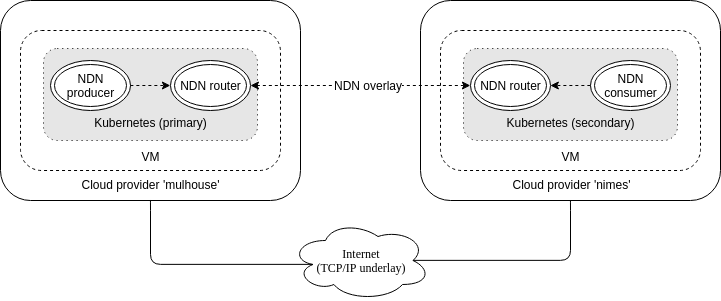
\includegraphics[width=\columnwidth]{Images/high-level-network-design.png}
\caption{High-level network design.}
\label{fig:high-level-network-design}
\end{figure}

In our high-level network design (figure \ref{fig:high-level-network-design}) we have three different virtual functions for NDN nodes. The producer is assigned the function to make data available in the NDN network. The consumer is assigned to request data from the producer. However, in NDN, any node that has named data, can reply to interest requests. So the producer and consumer functions are interchangeable. The router's function is to forward interest packets between the two cloud providers. This forwarding is done in the NDN overlay, which runs on top of the internet (underlay). These NDN functions are deployed via a Kubernetes cluster (section \ref{overview-virtualization}), spread over the two conceptual cloud providers; ('mulhouse' and 'nimes'). These cloud providers are spread geographically in order to provide users with their regional NDN cache. Kubernetes can be used to keep a central control over the NDN network, where pods (containers) can be created, removed and managed. These pods are spawned from images and custom tailored for their specific network function, as described in section \ref{overview-virtualization}. In summary; resources can be scaled in or out by deploying more VMs. In order to provide users a local NDN cache, a regional cloud provider can be used to deploy a VM. By the use of Kubernetes, the NDN application (node) can be scaled in and out as well. Where each NDN node can be responsible for caching/forwarding a different subset of the naming hierarchy. However, cache misses are expensive since they require a rebuild of the cache, which puts load on the original publisher of the data; SeaDataCloud. Which is what we want to prevent. Therefore, pods preferably are configured with persistent data volumes (section \ref{overview-virtualization}), on which the cached data can be stored outside of the container. Kubernetes can also load-balance requests between a set of pods. However, if these pods don't share the same persistent cached data, cache misses will occur, which results in performance degradation.

\subsection{Deploying an NDN network (McCabe and TOSCA)}
% Use relationships as defined by McCabe
\label{planning-deploying}
Now that the network analysis, design and architecture are defined, a deployment strategy is needed. The high-level design (figure \ref{fig:high-level-network-design}) needs to become deployable with a scalable method. Scalable in this context means that a single deployment strategy can be used for different cloud providers. Furthermore, as defined in the scope (section \ref{introduction-scope}) if the infrastructure scales out, the effort for managing a larger infrastructure should be equal. As described in section \ref{overview-tosca}, TOSCA is a standard to describe the complete life cycle of an infrastructure. There is a growing support for TOSCA template descriptions in cloud providers. Having a single set of template descriptions for deployment benefits portability and reproducibility of an infrastructure on different cloud providers.

\begin{figure}[H]
\centering
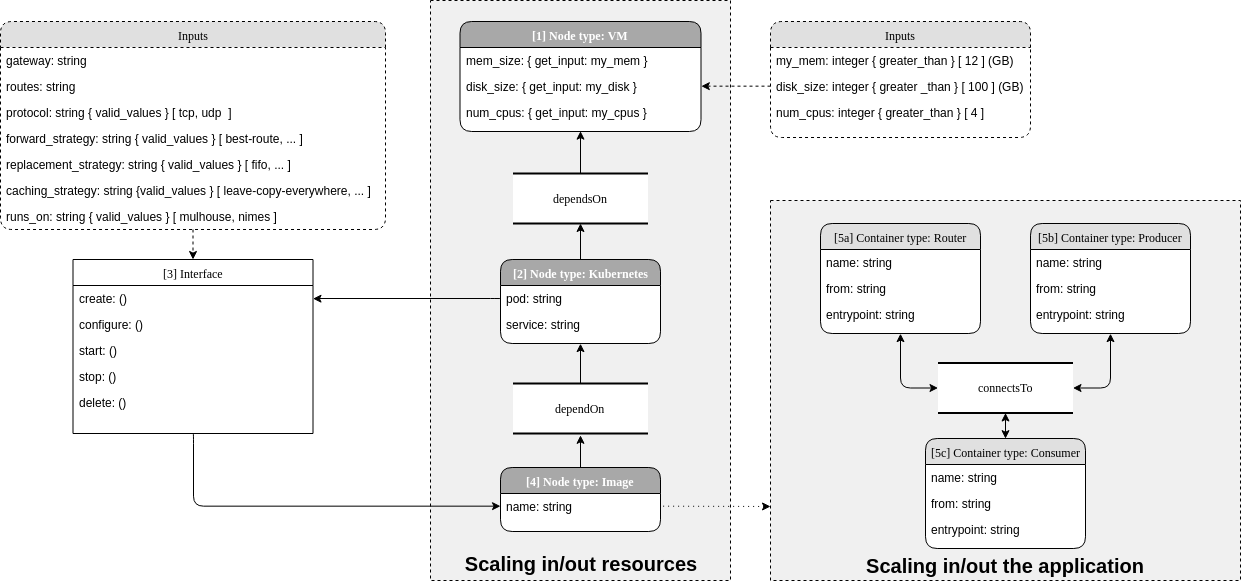
\includegraphics[width=\columnwidth]{Images/tosca-diagram.png}
\caption{TOSCA diagram.}
\label{fig:tosca-diagram}
\end{figure}

In figure \ref{fig:tosca-diagram} a TOSCA diagram is illustrated. This diagram represents an abstract template description of the TOSCA relationships, in which the grey rectangular boxes are the core scalability factors. As described in section \ref{overview-tosca}, TOSCA consists out of several types; nodes, relationships and interfaces. The scaling properties are highlighted in the rectangular areas. The left area, highlighted as 'scaling in/out resources' contains a dependency chain of several NDN functions. This dependency chain is also depicted numerically. Before a pod can be deployed on Kubernetes (step 2 to 5), a VM needs to exist (step 1). This is described by the 'dependsOn' relationship. Furthermore, with the requirements defined in section \ref{planning-requirements}, input constraints are described. These constraints are used by the orchestrator to make sure that the NDN infrastructure has sufficient resources available to operate. Once a VM is deployed the dependency for Kubernetes is satisfied, thus Kubernetes can then be setup (step 2). Kubernetes can then deploy pods by the use of interfaces (step 3). These interfaces feed the containers with environment variables such as the gateway, a list of routes, the transport protocol for NDN, the NDN strategies and on which Kubernetes node this pod should run. The environment variables are given to the interface via the TOSCA inputs. These environment variables are then used by scripts that run inside the pods to setup NDN. Several constraints are set for these environment variables such as which valid transport protocols can be used for NDN, which NDN strategies are valid and which nodes are available. These constraints are defined with e.g. 'valid\_values' or 'greater\_than' definitions. These constraints help to guide the orchestrator to verify the inputs that are given for the template description. As illustrated in the second gray area 'scaling in/out the application', several pods can be instantiated (step 5a, 5b and 5c) from the image (step 4). These pods enable the NDN functions as described in section \ref{planning-architecture}. These pods establish the NDN network and therefore are connected via the 'connectsTo' relationship. This network expands over to other Kubernetes nodes in the cluster due to the use of the Kubernetes built-in overlay network.

\subsection{Proof of concept}
\label{planning-poc}
With the methodology defined, in which scalability and performance requirements are met and a method for deployment is described, a proof of concept was used to test the methodology. The orchestrators mentioned in section \ref{overview-tosca} are still in a prototype phase. Therefore, in our proof of concept we deployed the VMs and Kubernetes nodes manually. In practice the life cycle of the Kubernetes pods are managed by a TOSCA orchestrator. Without having a TOSCA orchestrator available, steps 2 through 5 in figure \ref{fig:tosca-diagram} were be carried out by Kubernetes exclusively. This was done by defining the configuration properties of the pods manually\footnote{\url{https://github.com/AquaL1te/rp2/blob/master/Kubernetes/expanded-cluster.yml}}. These properties include the NDN function name, e.g. router, producer or consumer. And also includes the routes (NDN prefixes) and the associated NDN face with the transport protocol to use (TCP or UDP). These parameters were then inserted into the NDN FIB by the scripts that were executed inside the pod\footnote{\url{https://github.com/AquaL1te/rp2/blob/master/Docker/producer/docker-entrypoint.sh}}. The NDN strategies were also configured by these same scripts. Furthermore, if it's not defined where a pod should be running, Kubernetes will make this decision itself, based on the known resources in the Kubernetes cluster. If for example a Kubernetes node has more memory to spare than other nodes, then Kubernetes will likely decide to spawn the pod there. This Kubernetes node could potentially run in a cloud provider, located in another geographical area. Since the purpose is to provide data distribution through the use of NDN, locality becomes a key factor. Therefore, a pod is specifically assigned to a Kubernetes node in order to provide in-network caching in a specific geographical area.

\subsection{Results}
As a result, the NDN infrastructure life cycle can be managed from Kubernetes. Our proof of concept lacks a TOSCA orchestrator. Therefore, scaling in or out resources to other cloud provider is not demonstrated. However, scaling in or out the NDN application is demonstrated. This method allows to reconfigure an NDN infrastructure in VNF-style by interacting with Kubernetes as the orchestrator. Therefore, the YAML configuration of Kubernetes acts as the TOSCA template description and Kubernetes, which executes this configuration, acts as the orchestrator. In practice the Kubernetes configuration would be generated based on the TOSCA template descriptions and e.g. DRIP would act as the orchestrator. In effect, the NDN containers are spawned as VNFs which provides scalable management of the NDN network.